\documentclass[aspectratio=169,handout,bigger]{beamer}

\usepackage{minted}
\usepackage[utf8]{inputenc}
\usepackage{graphicx}
\usepackage[T1,T2A]{fontenc}
\usepackage[american,russian]{babel}

\usepackage{tikz}
\usetikzlibrary{shapes,arrows,chains,calc,fit,matrix}
\tikzstyle{line}=[draw]
\tikzstyle{arrow}=[draw]

%% -------------------------------------------------------------------------- %%

\mode<presentation>{
  \usetheme{default}
}

\setbeamertemplate{navigation symbols}{}
\setbeamertemplate{footline}[frame number]

\newcommand{\comment}[1]{}

%% -------------------------------------------------------------------------- %%

\title{
\includegraphics[height=.15\textheight]{logo}}
\author{Пользовательская автоматизация\newlineпрофессиональных веб-приложений\newlineна Lua}
\institute{Александр Гладыш\newline@agladysh}
\date{Lua in Moscow\\Сентябрь 2016}

%% -------------------------------------------------------------------------- %%

\begin{document}

\maketitle

%% -------------------------------------------------------------------------- %%

\section{Задача}

%% -------------------------------------------------------------------------- %%

\begin{frame}{Профессиональные приложения}

Профессиональное приложение:

\begin{itemize}
\item Для профессионалов, глубоко владеющих предметной областью
\item Которые в большинстве своём не айтишники
\end{itemize}

Примеры:

\begin{itemize}
\item CAD'ы
\item Приложения для управления бизнес-логикой "больших" систем
\item Бэкофисы сложных проектов
\item и так далее
\end{itemize}

\end{frame}

%% -------------------------------------------------------------------------- %%

\begin{frame}{Конкретика}

\begin{itemize}
\item ТАИС разрабатывает профессиональное ПО для гражданской авиации
\item Глубокая и обширная предметная область с длинной историей
\item Требует профессионального обучения пользователей
\end{itemize}

\end{frame}

%% -------------------------------------------------------------------------- %%

\begin{frame}{Пользовательский интерфейс предыдущего поколения}

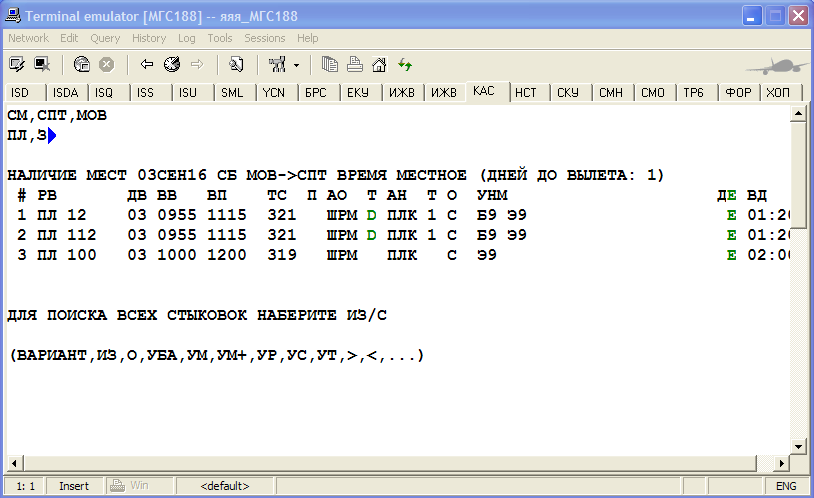
\includegraphics[width=.90\textwidth]{temul}

\end{frame}

%% -------------------------------------------------------------------------- %%

\begin{frame}{Перспективный пользовательский интерфейс}

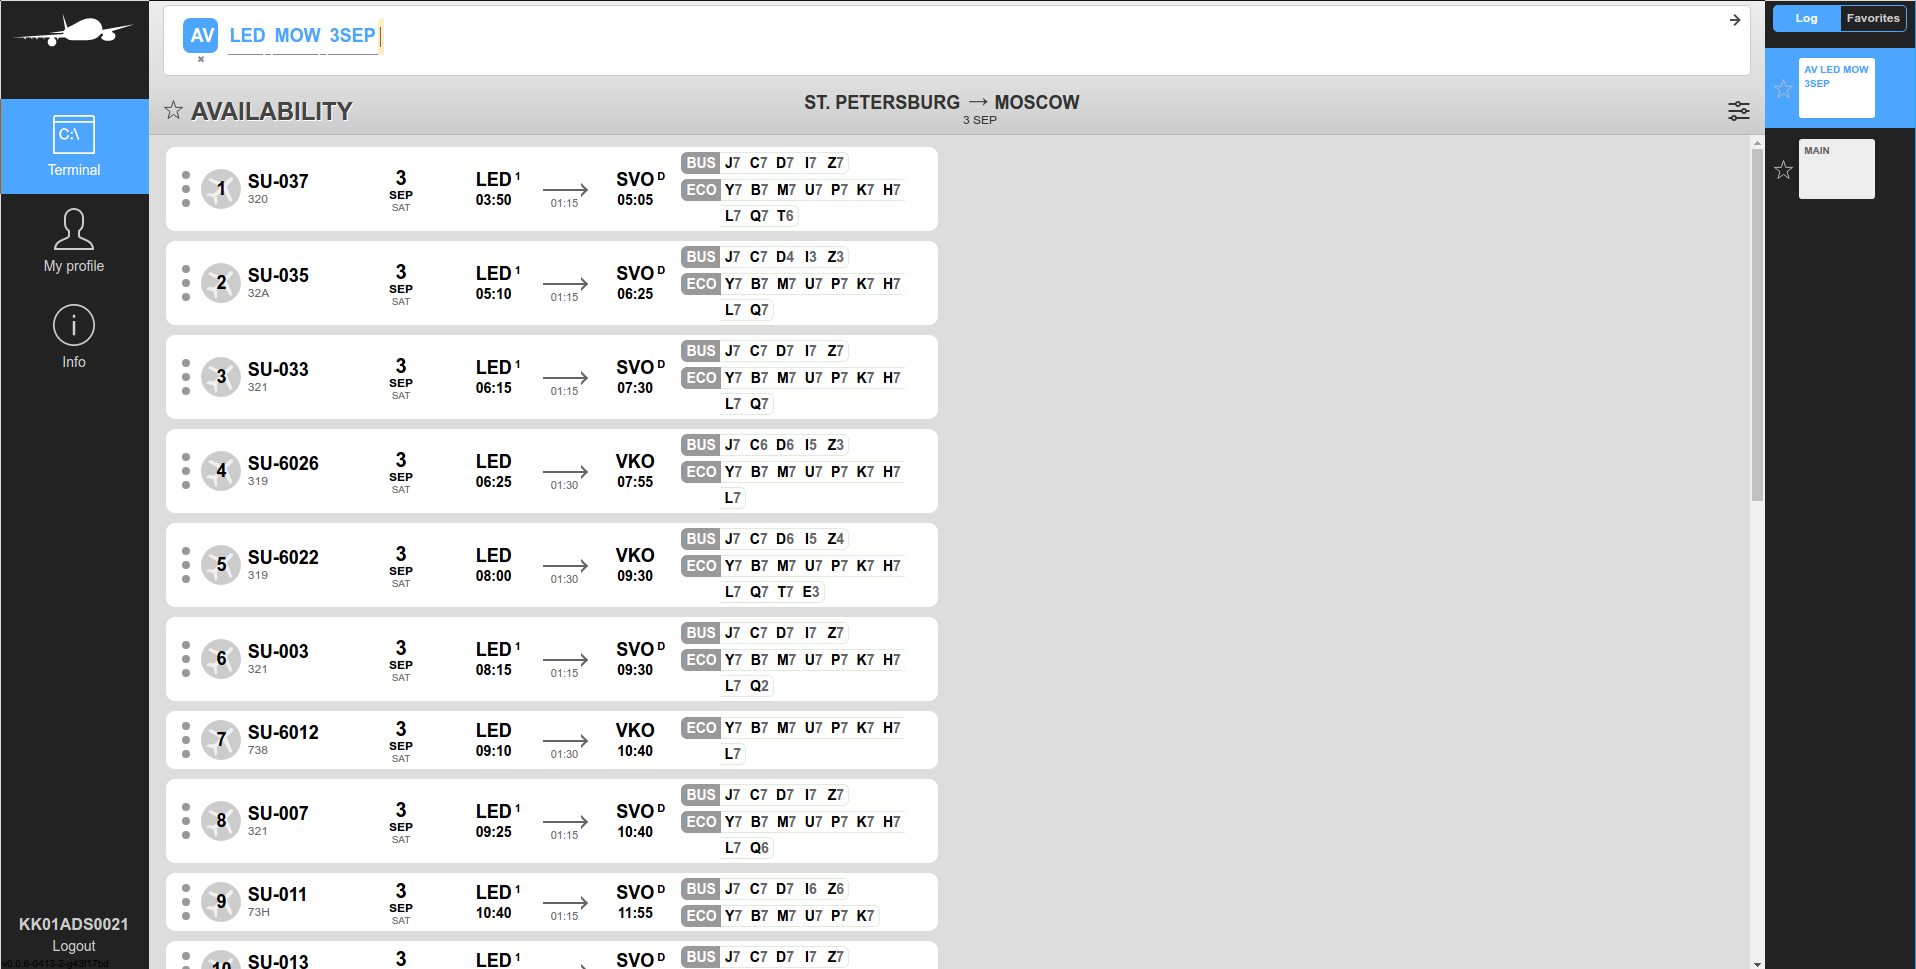
\includegraphics[width=.90\textwidth]{twt}

\end{frame}

%% -------------------------------------------------------------------------- %%

\begin{frame}{Многослойная система}

\begin{tikzpicture}

\node (client) {Клиент};
\node (server) [below of=client] {REST-сервер};
\node (sig) [below of=server] {Легаси SOAP-процессор};
\node (crs) [below of=sig] {CRS};
\node (external) [below of=crs] {Внешние системы};

\draw [arrow] (client) -> (server);
\draw [arrow] (server) -> (sig);
\draw [arrow] (sig) -> (crs);
\draw [arrow] (crs) -> (external);

\end{tikzpicture}

\end{frame}

%% -------------------------------------------------------------------------- %%

\begin{frame}{Поток сообщений}

\begin{tikzpicture}

\node (command) {Пользовательская команда};
\node (rpcrequest) [below of=command] {Запрос REST};
\node (soaprequest) [below of=rpcrequest] {Запрос SOAP};
\node (etc) [below of=soaprequest] {...};
\node (external) [below of=etc] {Запросы ко внешним системам};

\draw [arrow] (command) -> (rpcrequest);
\draw [arrow] (rpcrequest) -> (soaprequest);
\draw [arrow] (soaprequest) -> (etc);
\draw [arrow] (etc) -> (external);

\end{tikzpicture}

\end{frame}

%% -------------------------------------------------------------------------- %%

\begin{frame}{Задачи}

\begin{itemize}
\item Автоматизация редких но сложных операций пользователя-эксперта
\item В дальнейшем --- удобное API для более широкого круга пользователей
\end{itemize}

\end{frame}

%% -------------------------------------------------------------------------- %%

\section{Решение}

%% -------------------------------------------------------------------------- %%

\begin{frame}{Почему макросы на клиенте?}

\begin{itemize}
\item Запускать код пользователя на сервере — головная боль
\item Особенно если уже есть система пользовательских команд
\item Даже если её нет — у вас же есть серверное HTTP-API, правда?
\end{itemize}

\end{frame}

%% -------------------------------------------------------------------------- %%

\begin{frame}{Почему Lua?}

\begin{itemize}
\item JavaScript тяжело изолировать от "кишок" проекта
\item Lua легко изолировать
\item Сам факт использования другого языка делает дизайн API чище
\item Lua легче освоить непрограммистами
\end{itemize}

\end{frame}

%% -------------------------------------------------------------------------- %%

\begin{frame}{Внешний вид: редактор скриптов}

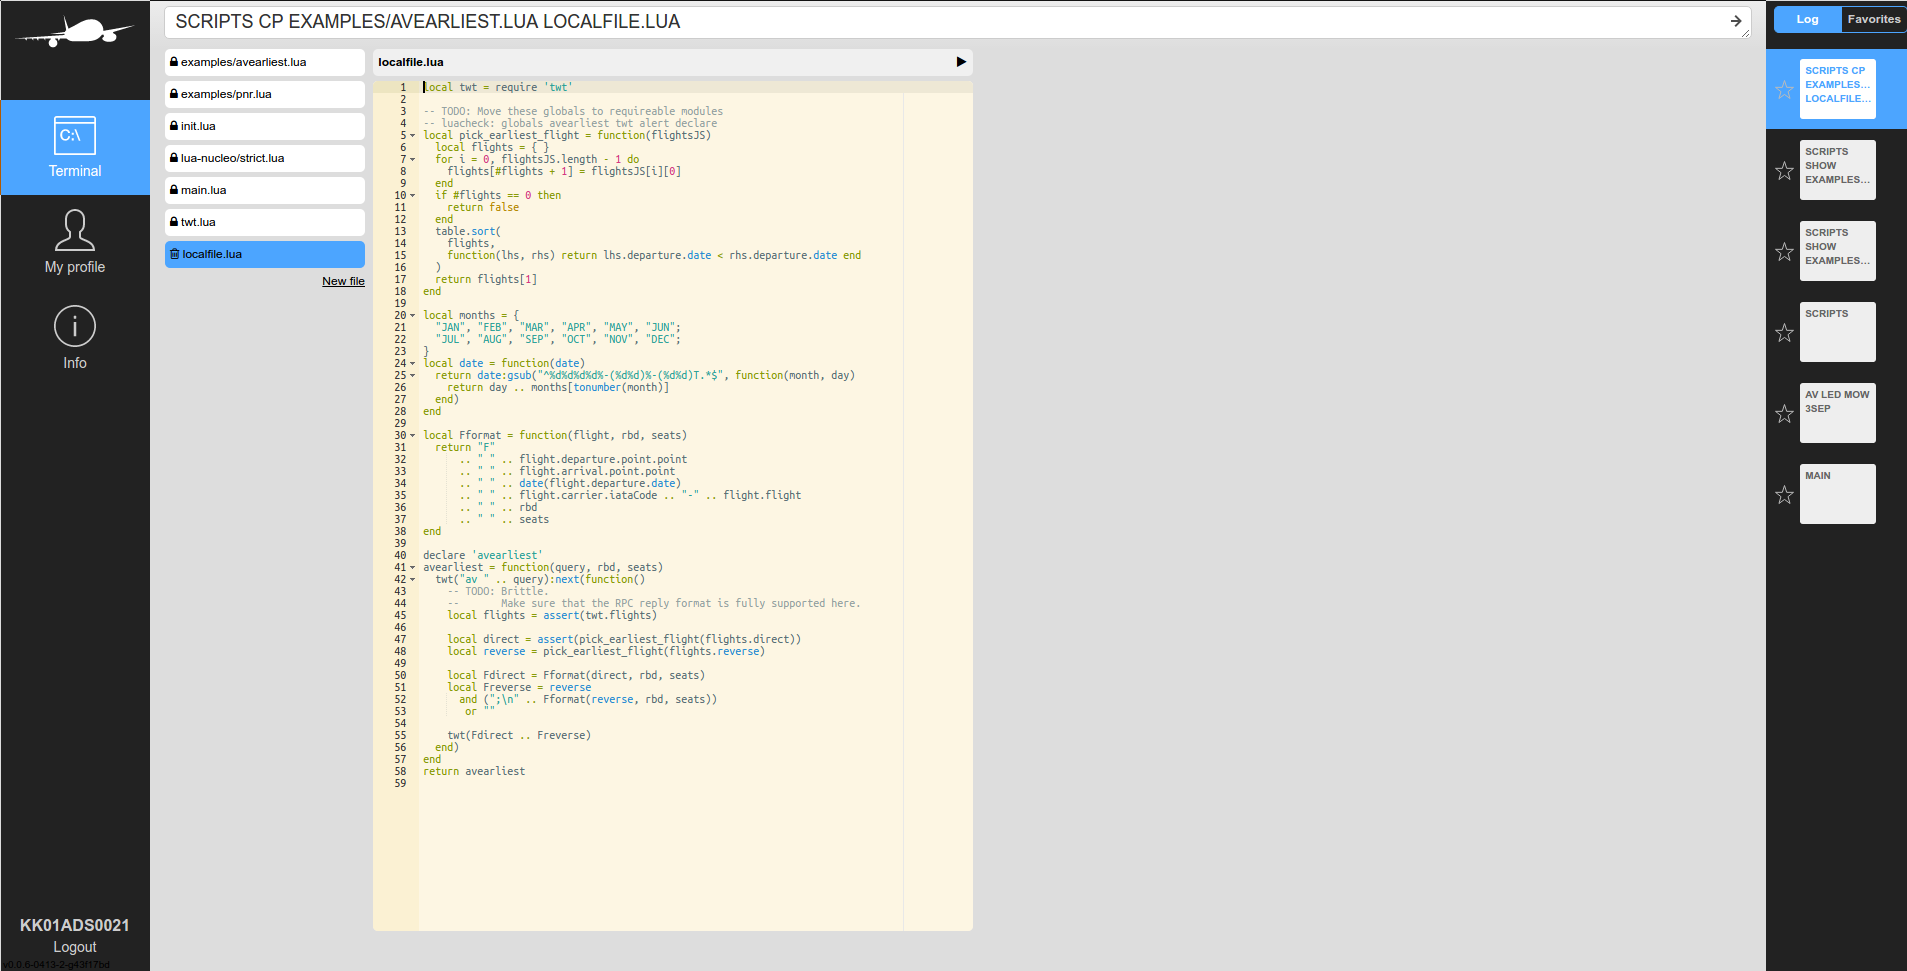
\includegraphics[width=.90\textwidth]{scripts}

\end{frame}

%% -------------------------------------------------------------------------- %%

\begin{frame}{Внешний вид: команда}


\includegraphics[width=.90\textwidth]{command}

\end{frame}

%% -------------------------------------------------------------------------- %%

\begin{frame}{Внешний вид: результат выполнения}

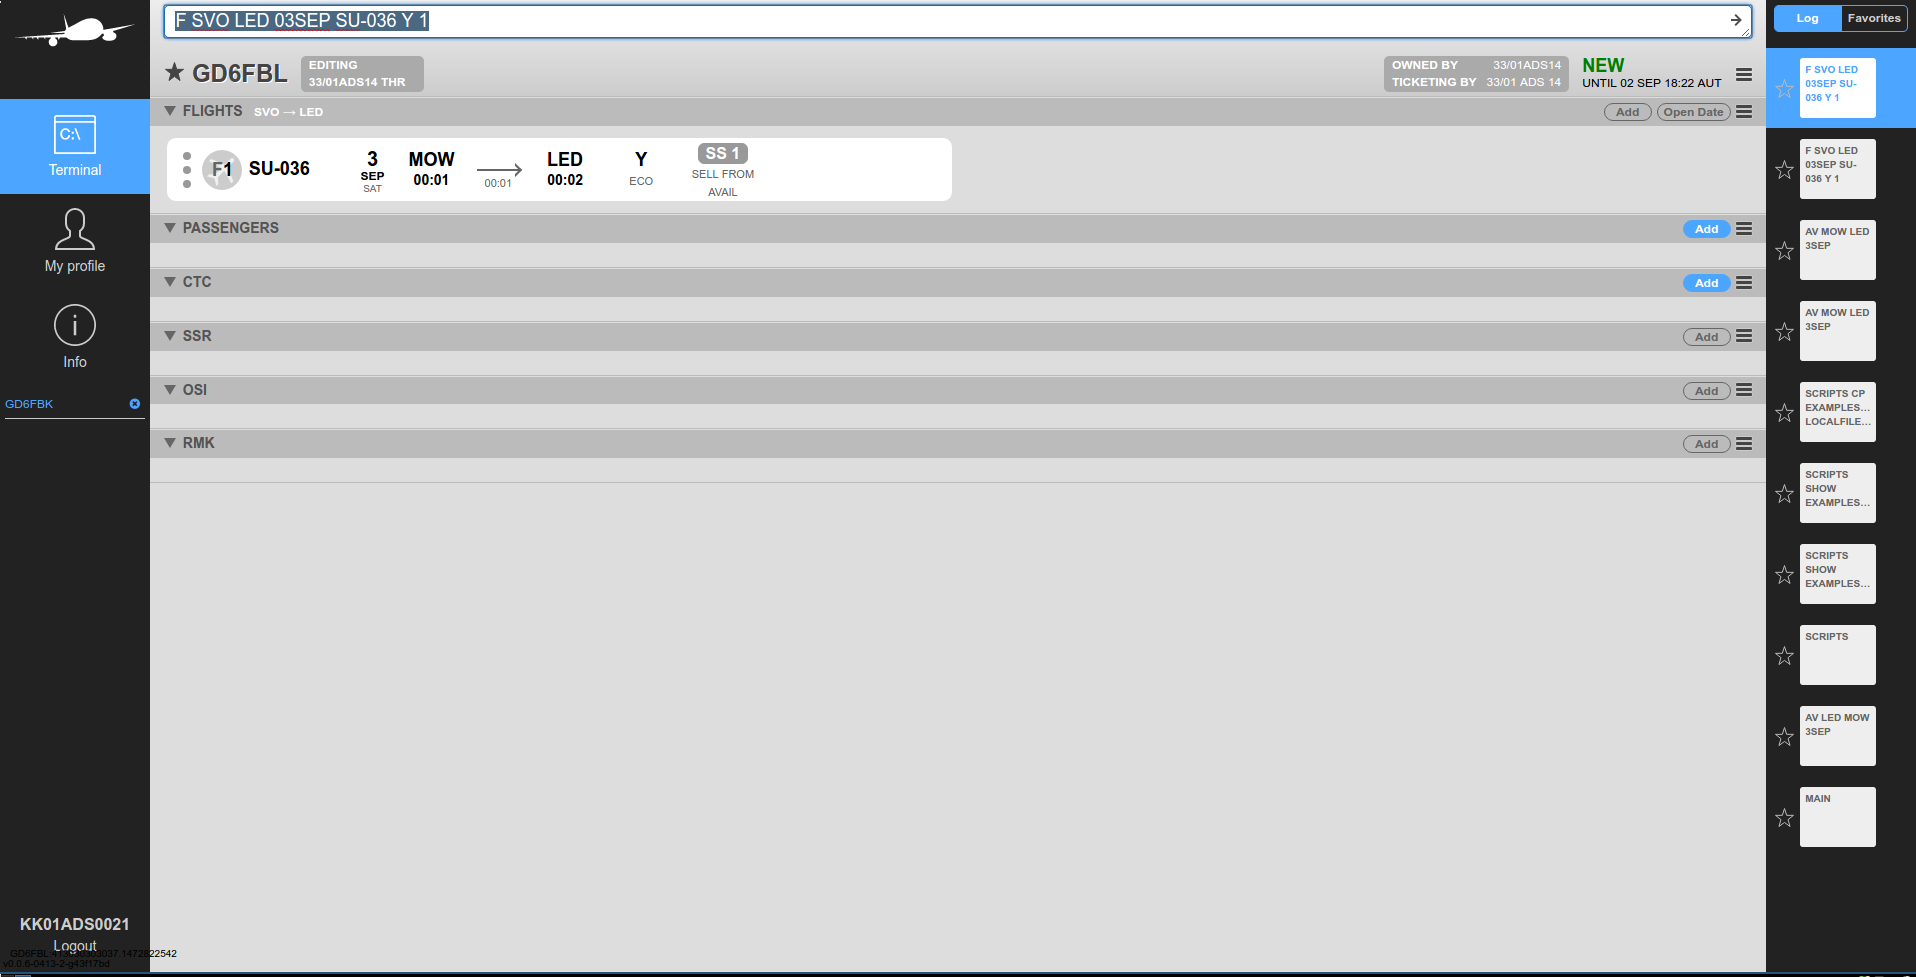
\includegraphics[width=.90\textwidth]{result}

\end{frame}

%% -------------------------------------------------------------------------- %%

\begin{frame}{Lua в браузере: варианты}

\begin{itemize}
\item lua.vm.js
\item moonshine.js
\item lua5.1.js
\item starlight
\item ... и многие другие.
\end{itemize}

См. также: Sailor MVC.

\end{frame}

%% -------------------------------------------------------------------------- %%

\begin{frame}{Наш стек}

\begin{itemize}
\item lua.vm.js
\item Маленькая самописная библиотека для VFS
\item ACE (brace)
\item webpack
\end{itemize}

\end{frame}

%% -------------------------------------------------------------------------- %%

\begin{frame}[fragile]{Немного кода}

\begin{minted}{javascript}
var LuaVM = require('lua.vm.js');

var execute = function(code) { return this.lua_.execute(code); };
var provideModule = function(name, value) {
  this.lua_._G.get("package").get("loaded").set(name, value);
};

var Vm = function() { this.lua_ = new LuaVM.Lua.State(); };

Vm.prototype = {
  execute: execute,
  provideModule: provideModule,
  constructor: Vm
};
module.exports = Vm;
\end{minted}

\end{frame}

%% -------------------------------------------------------------------------- %%

\begin{frame}{Что дальше?}

\begin{itemize}
\item Технически — Lua в браузере отлично работает и выполняет свои задачи.
\item Главное — это удобство использования, а это уже вопрос дизайна API.
\end{itemize}

\end{frame}

%% -------------------------------------------------------------------------- %%

\section{Вопросы?}

%% -------------------------------------------------------------------------- %%

\begin{frame}{Вопросы?}

Alexander Gladysh\newline
@agladysh

\end{frame}

%% -------------------------------------------------------------------------- %%

\end{document}

%% -------------------------------------------------------------------------- %%
